\chapter{Dynamic programming decision trees in practice}\label{sec:exps-dt}

In this section, we empirically demonstrate strong properties of DPDT trees. 
The first part of our experiments focuses on the quality of solutions obtained by DPDT for objective Eq.\ref{eq:suplearning} compared to greedy and optimal trees. We know by theorems \ref{prop:cart} and \ref{thm:better_greedy} that DPDT trees should find better solutions than greedy algorithms for certain problems; but what about real problems?
After showing that DPDT can find optimal trees by considering much less solutions and thus performing orders of magnitude less operations, we will study the generalization capabilities of the latter: do DPDT trees label unseen data accurately?

\section{DPDT optimizing capabilities}
\begin{table}[ht]
    \centering
    \tiny
    \caption{Comparison of train accuracies of depth-3 trees and number of operations on classification tasks. For DPDT and Top-B, ``light'' configurations have split function parameters (8, 1, 1) ``full'' have parameters (8, 8, 8). We also include the mean train accuracy over 5 deep RL runs. \textbf{Bold} values are optimal accuracies and {\color{blue} blue} values are the largest non-optimal accuracies.}
    \label{tab:tree_comparison_combined}
    \begin{tabular}{l|cc||cc|cc|cc|c||cc|cc|cc}
    \toprule
    & & & \multicolumn{7}{c||}{\textbf{Accuracy}} & \multicolumn{6}{c}{\textbf{Operations}}\\
    \midrule
    & & & Opt & Greedy & \multicolumn{2}{c|}{DPDT} & \multicolumn{2}{c|}{Top-B} & \multicolumn{1}{c||}{Deep RL} & Opt & Greedy & \multicolumn{2}{c|}{DPDT} & \multicolumn{2}{c}{Top-B}\\
    \textbf{Dataset} & N & p & Quant-BnB & CART & light & full & light & full & Modified DQN & Quant-BnB & CART & light & full & light & full \\
    % version précédente rempplacée par les 3 lignes ci-dessus :
    % & & & \multicolumn{2}{c|}{\textbf{Accuracy}} & \multicolumn{2}{c|}{DPDT} & \multicolumn{2}{c|}{Top-B} & \multicolumn{1}{c||}{Deep RL} & \multicolumn{2}{c|}{\textbf{Operations}} & \multicolumn{2}{c|}{DPDT} & \multicolumn{2}{c}{Top-B}\\
    % \textbf{Dataset} & N & p & Opt & Greedy & light & full & light & full & Custard & Opt & Greedy & light & full & light & full \\
    \midrule
    room & 8103 & 16 & \textbf{0.992} & 0.968 & \color{blue} 0.991 & \textbf{0.992} & 0.990 & \textbf{0.992} & 0.715 &$10^6$ & 15 & 286 & 16100 & 111 & 16100 \\
    bean & 10888 & 16  & \textbf{0.871} & 0.777 & 0.812 & \color{blue} 0.853 & 0.804 & 0.841 & 0.182 & 5$\cdot 10^6$ & 15 & 295 & 25900 & 112 & 16800 \\
    eeg & 11984 & 14  & \textbf{0.708} & 0.666 & 0.689 & \color{blue} 0.706 & 0.684 & 0.699 & 0.549 & 2$\cdot 10^6$ & 13 & 289 & 26000 & 95 & 11000 \\
    avila & 10430 & 10  & \textbf{0.585} & 0.532 & \color{blue}0.574 & \textbf{0.585} & 0.563 & 0.572 & 0.409 & 3$\cdot 10^7$ & 9 & 268 & 24700 & 60 & 38900 \\
    magic & 15216 & 10 & \textbf{0.831} & 0.801 & 0.822 & \color{blue} 0.828 & 0.807 & 0.816 & 0.581 &6$\cdot 10^6$ & 15 & 298 & 28000 & 70 & 4190 \\
    htru & 14318 & 8  & \textbf{0.981} & 0.979 & 0.979 & \color{blue}0.980 & 0.979 & \color{blue}0.980 & 0.860 & 6$\cdot 10^7$ & 15 & 295 & 25300 & 55 & 2180 \\
    occup. & 8143 & 5 & \textbf{0.994} & 0.989 & 0.991 & \textbf{0.994} & 0.990 & \color{blue}0.992 & 0.647 & 7$\cdot 10^5$ & 13 & 280 & 16300 & 33 & 510 \\
    skin & 196045 & 3 & \textbf{0.969} & \color{blue}0.966 & \color{blue}0.966 & \color{blue}0.966 & \color{blue}0.966 & \color{blue}0.966 & 0.612 & 7$\cdot 10^4$ & 15 & 301 & 23300 & 20 & 126 \\
    fault & 1552 & 27 & \textbf{0.682} & 0.553 & 0.672 & \color{blue}0.674 & 0.672 & 0.673 & 0.303 & 9$\cdot 10^8$ & 13 & 295 & 24200 & 111 & 16800 \\
    segment & 1848 & 18 & \textbf{0.887} & 0.574 & 0.812 & \color{blue}0.879 & 0.786 & 0.825 & 0.137 & 2$\cdot 10^6$ & 7 & 220 & 16300 & 68 & 11400 \\
    page & 4378 & 10 &  \textbf{0.971} & 0.964 & \color{blue}0.970 & \color{blue}0.970 & 0.964 & 0.965 & 0.902 &$10^7$ & 15 & 298 & 22400 & 701 & 4050 \\
    bidding & 5056 & 9  & \textbf{0.993} & 0.981 & \color{blue}0.985 & \textbf{0.993} & 0.985 & \textbf{0.993} & 0.810 & 3$\cdot 10^5$ & 13 & 256 & 9360 & 58 & 2700 \\
    raisin & 720 & 7 & \textbf{0.894} & 0.869 & 0.879 & \color{blue}0.886 & 0.875 & 0.883 & 0.509 & 4$\cdot 10^6$ & 15 & 295 & 20900 & 48 & 1440 \\
    rice & 3048 & 7 & \textbf{0.938} & 0.933 & 0.934 & \color{blue}0.937 & 0.933 & 0.936 & 0.519 & 2$\cdot 10^7$ & 15 & 298 & 25500 & 49 & 1470 \\
    wilt & 4339 & 5 & \textbf{0.996} & 0.993 & 0.994 & \color{blue}0.995 & 0.994 & 0.994 & 0.984 &3$\cdot 10^5$ & 13 & 274 & 11300 & 33 & 465 \\
    bank & 1097 & 4 & \textbf{0.983} & 0.933 & 0.971 & \color{blue}0.980 & 0.951 & 0.974 & 0.496 & 6$\cdot 10^4$ & 13 & 271 & 7990 & 26 & 256 \\
% ancienne présentation :
    %% room & 8103 & 16 & 0.992 & 0.968 & 0.991 & 0.992 & 0.990 & 0.992 & 0.715 & 1.34e+06 & 15 & 286 & 16100 & 111 & 16100 \\
    %% bean & 10888 & 16  & 0.871 & 0.777 & 0.812 & 0.853 & 0.804 & 0.841 & 0.182 & 4.66e+06 & 15 & 295 & 25900 & 112 & 16800 \\
    %% eeg & 11984 & 14  & 0.708 & 0.666 & 0.689 & 0.706 & 0.684 & 0.699 & 0.549 & 1.50e+08 & 13 & 289 & 26000 & 95 & 11000 \\
    %% avila & 10430 & 10  & 0.585 & 0.532 & 0.574 & 0.585 & 0.563 & 0.572 & 0.409 & 2.70e+07 & 9 & 268 & 24700 & 60 & 38900 \\
    %% magic & 15216 & 10 & 0.831 & 0.801 & 0.822 & 0.828 & 0.807 & 0.816 & 0.581 &5.71e+06 & 15 & 298 & 28000 & 70 & 4190 \\
    %% htru & 14318 & 8  & 0.981 & 0.979 & 0.979 & 0.980 & 0.979 & 0.980 & 0.860 & 6.22e+07 & 15 & 295 & 25300 & 55 & 2180 \\
    %% occupancy & 8143 & 5 & 0.994 & 0.989 & 0.991 & 0.994 & 0.990 & 0.992 & 0.647 & 6.81e+05 & 13 & 280 & 16300 & 33 & 510 \\
    %% skin & 196045 & 3 & 0.969 & 0.966 & 0.966 & 0.966 & 0.966 & 0.966 & 0.612 & 71100 & 15 & 301 & 23300 & 20 & 126 \\
    %% fault & 1552 & 27 & 0.682 & 0.553 & 0.672 & 0.674 & 0.672 & 0.673 & 0.303 & 9.32e+08 & 13 & 295 & 24200 & 111 & 16800 \\
    %% segment & 1848 & 18 & 0.887 & 0.574 & 0.812 & 0.879 & 0.786 & 0.825 & 0.137 & 2.13e+06 & 7 & 220 & 16300 & 68 & 11400 \\
    %% page & 4378 & 10 &  0.971 & 0.964 & 0.970 & 0.970 & 0.964 & 0.965 & 0.902 & 9.62e+06 & 15 & 298 & 22400 & 701 & 4050 \\
    %% bidding & 5056 & 9  & 0.993 & 0.981 & 0.985 & 0.993 & 0.985 & 0.993 & 0.810 & 2.69e+05 & 13 & 256 & 9360 & 58 & 2700 \\
    %% raisin & 720 & 7 & 0.894 & 0.869 & 0.879 & 0.886 & 0.875 & 0.883 & 0.509 & 3.98e+06 & 15 & 295 & 20900 & 48 & 1440 \\
    %% rice & 3048 & 7 & 0.938 & 0.933 & 0.934 & 0.937 & 0.933 & 0.936 & 0.519 & 2.08e+07 & 15 & 298 & 25500 & 49 & 1470 \\
    %% wilt & 4339 & 5 & 0.996 & 0.993 & 0.994 & 0.995 & 0.994 & 0.994 & 0.984 &3.20e+05 & 13 & 274 & 11300 & 33 & 465 \\
    %% bank & 1097 & 4 & 0.983 & 0.933 & 0.971 & 0.980 & 0.951 & 0.974 & 0.496 & 62500 & 13 & 271 & 7990 & 26 & 256 \\
    \bottomrule
    \end{tabular}
\end{table}
\begin{figure}
    \centering
    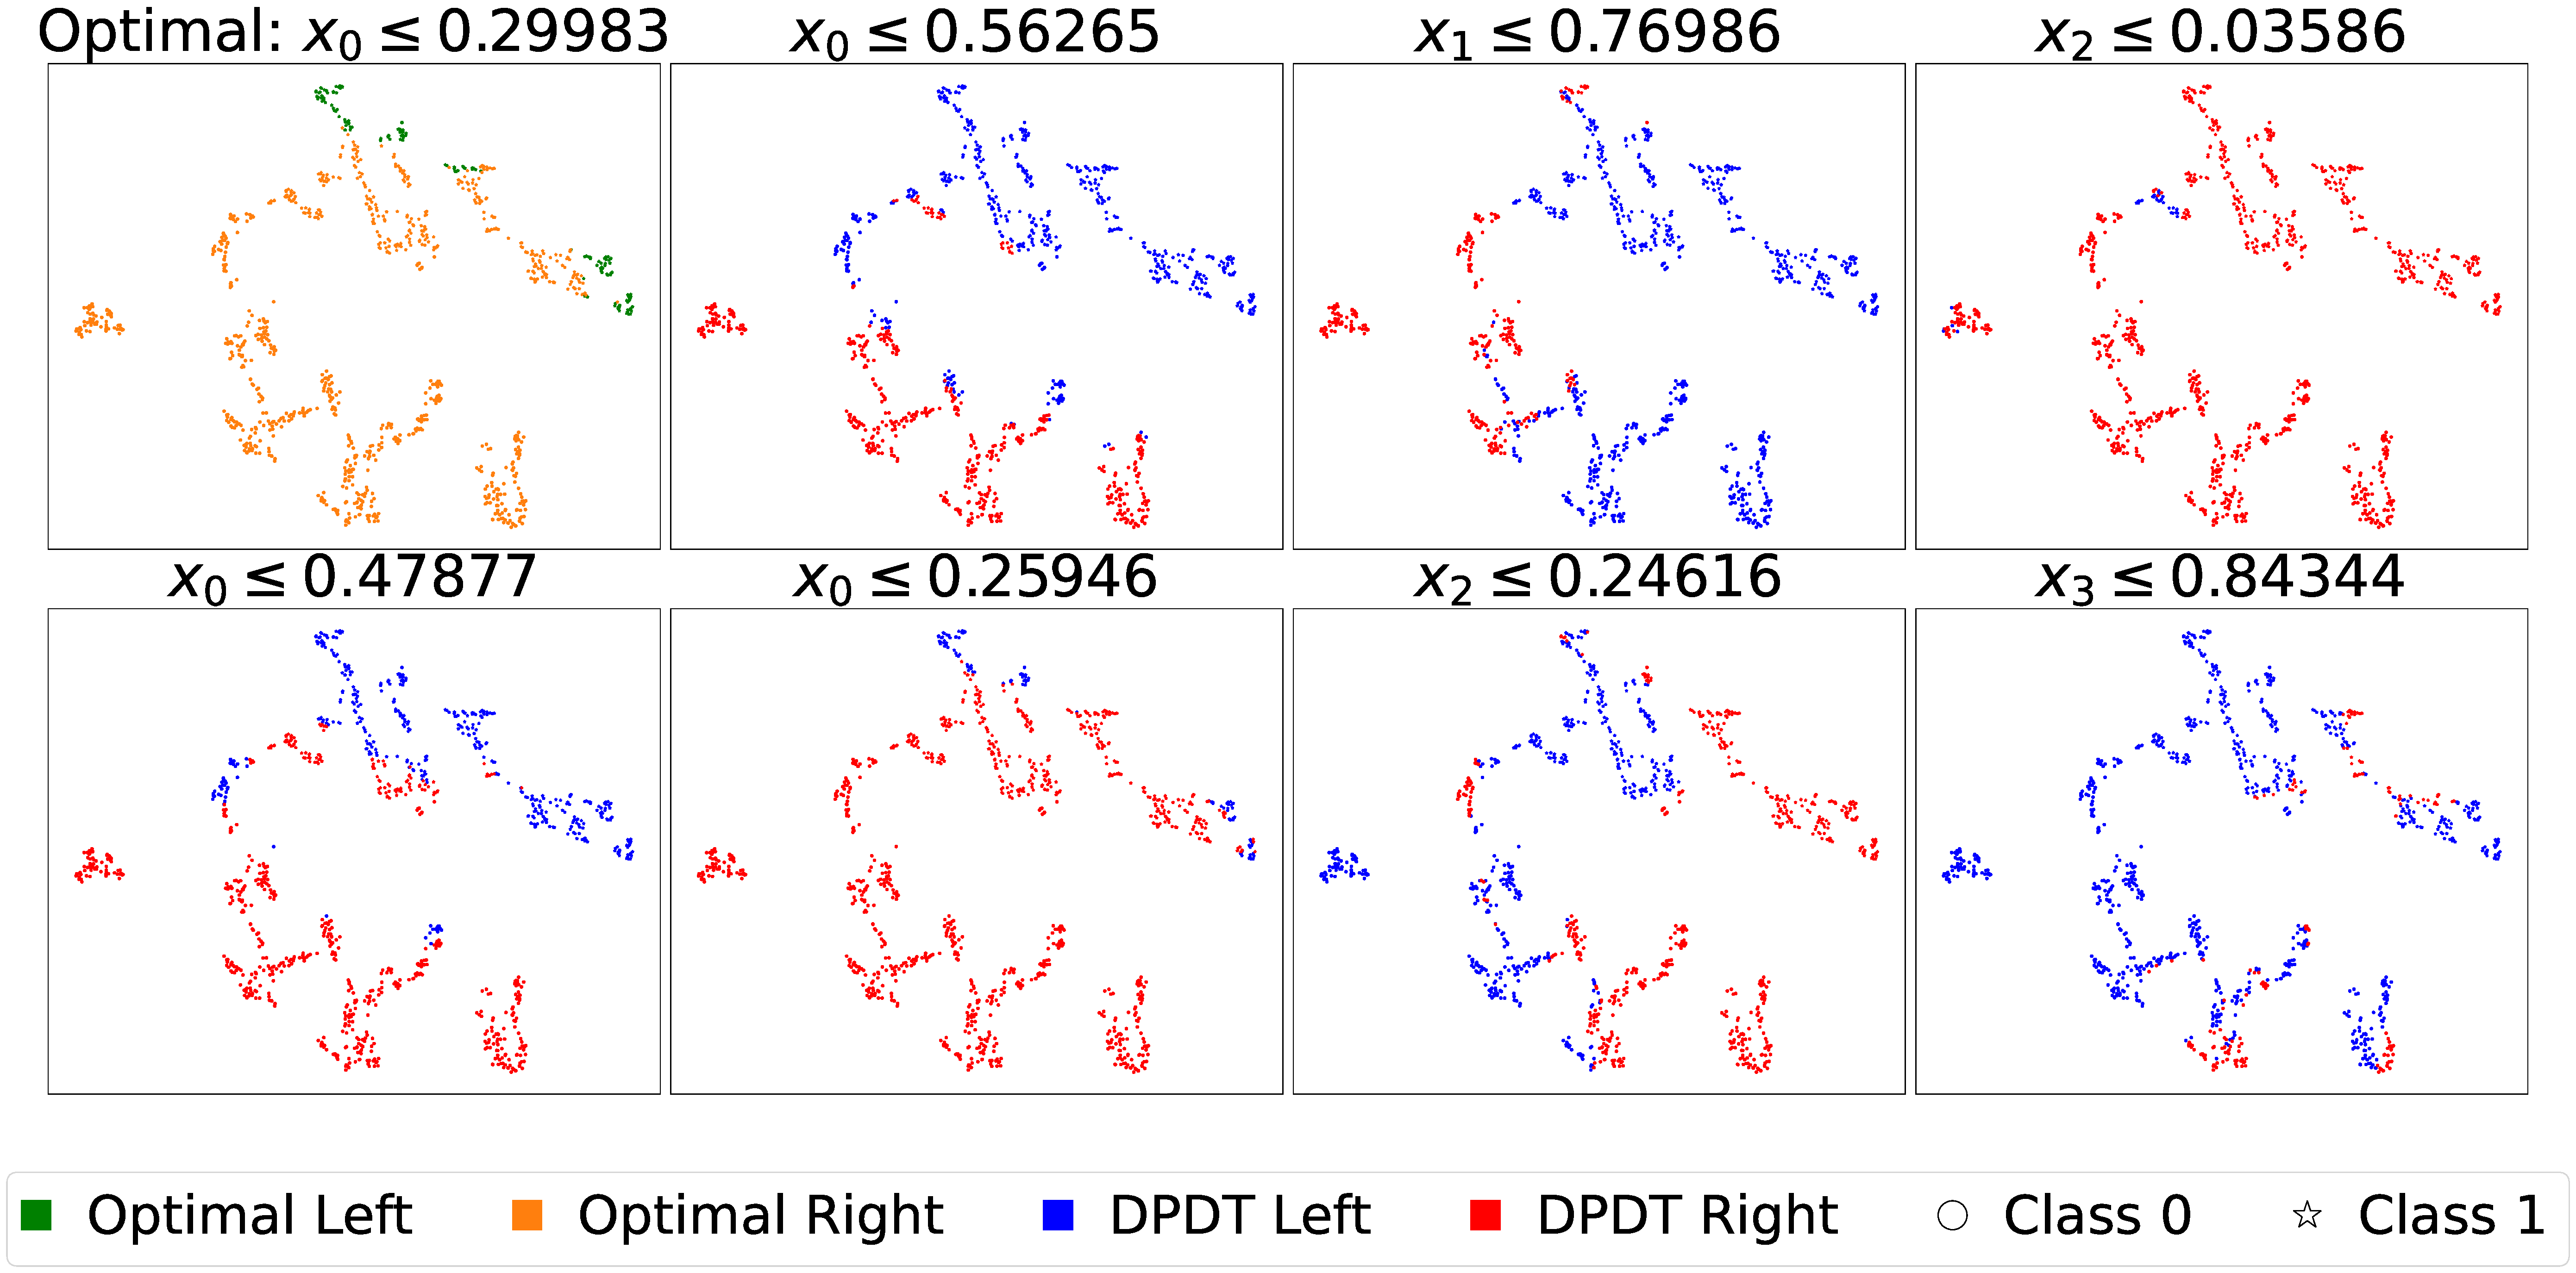
\includegraphics[width=1\linewidth]{images/figures/splits_tsne_combined.pdf}
    \caption{Root splits candidate obtained with DPDT compared to the optimal root split on the Bank dataset. Each split creates a partition of $p$-dimensional data that we projected in the $2$-dimensional space using t-SNE.}
    \label{fig:splits_dpdt}
\end{figure}
\begin{figure}
    \centering
    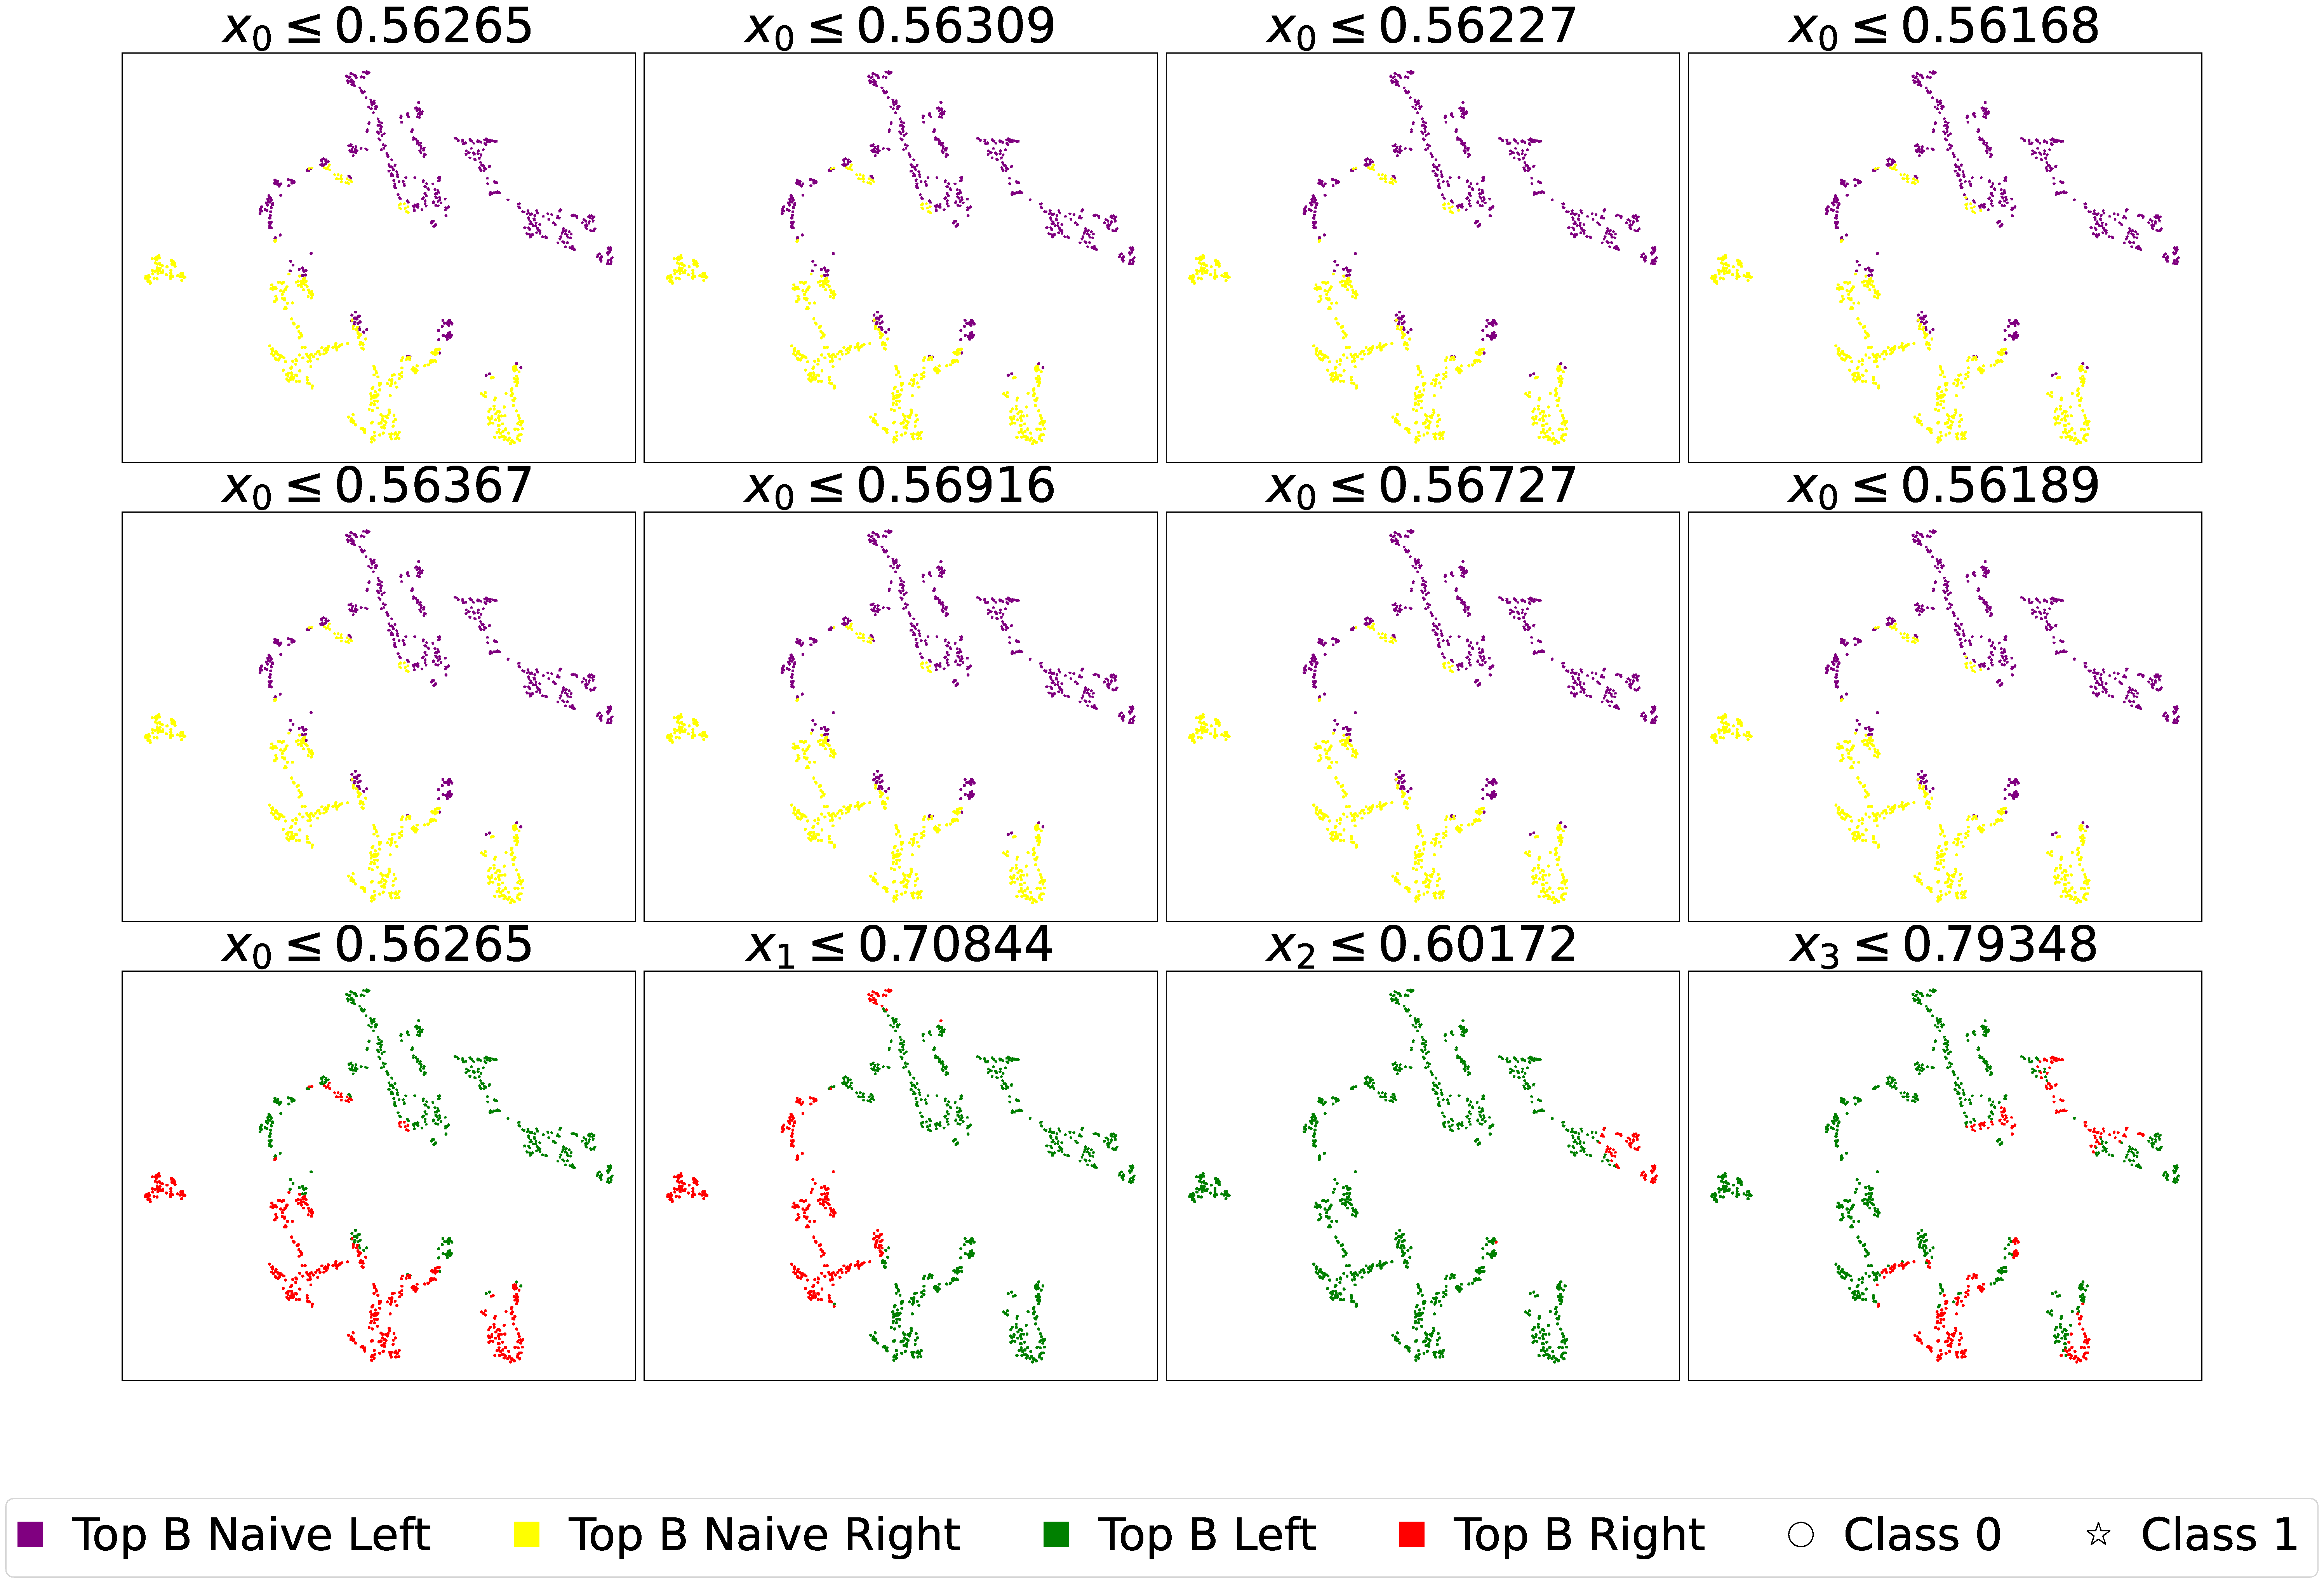
\includegraphics[width=1\linewidth]{images/figures/splits_tsne_combined_topk.pdf}
    \caption{Root splits candidate obtained with Top-B\cite{topk} on the Bank dataset. Each split creates a partition of $p$-dimensional data that we projected using t-SNE.}
    \label{fig:splits_topb}
\end{figure}

From an empirical perspective, it is key to evaluate DPDT training accuracy since optimal decision tree algorithms against which we wish to compare ourselves are designed to optimize the regularized training loss Eq.\ref{eq:suplearning}.

\subsection{Setup}
\paragraph{Metrics:} we are interested in the regularized training loss of algorithms optimizing Eq.\ref{eq:suplearning} with $\alpha=0$ and a maximum depth $D$. We are also interested in the number of key operations performed by each baseline, namely computing candidate split nodes for subsets of the training data. We disregard running times as solvers are implemented in different programming languages and/or using optimized code: operations count is more representative of an algorithm efficiency. We also qualitatively compare different decision trees root splits to some optimal root split.
\paragraph{Baselines:} we benchmark DPDT against greedy trees and optimal trees. For greedy trees we compare DPDT to CART \cite{breiman1984classification}. For optimal trees we compare DPDT to Quant-BnB \cite{quantbnb} which is the only solver specialized for depth 3 trees and continuous features. We also consider the non-greedy baseline Top-B \cite{topk}. Ideally, DPDT should have training accuracy close to the optimal tree while performing a number of operations close to the greedy algorithm. Furthermore, comparing DPDT to Top-B brings answers to which heuristic splits are better to consider. 

We use the CART algorithm implemented in \texttt{scikit-learn}~\cite{scikit-learn} in \texttt{CPython} with a maximum depth of 3. Optimal trees are obtained by running the \texttt{Julia} implementation of the Quant-BnB solver from~\cite{quantbnb} specialized in depth 3 trees for datasets with continuous features. We use a time limit of 24 hours per dataset. 
DPDT and Top-B trees are obtained with algorithm~\ref{alg:dpdt} implemented in pure \texttt{Python} and the calls to CART and Top-B most informative splits generating functions from section~\ref{sec:the-mdp} respectively.
We use the modified DQN from section~\ref{sec:topin} on classification POIBMDPs with $\zeta=1$ (we want to learn the best tree possible disregarding interpretability) and maximum depth control using rewards or termination signals.
\paragraph{Datasets:} we us the same datasets as the Quant-BnB paper~\cite{quantbnb}.

\subsection{Observations}

\paragraph{Near-optimality} Our experimental results demonstrate that unlike Deep RL, DPDT and Top-B approaches consistently improve upon greedy solutions while requiring significantly fewer operations than exact solvers. Looking at Table~\ref{tab:tree_comparison_combined}, we observe several key patterns:
first, light DPDT with 16 candidate root splits consistently outperforms the greedy baseline in all datasets. This shows that in practice DPDT can be strictly netter than CART outside of theorem \ref{thm:better_greedy} assumptions. 
Second, when comparing DPDT to Top-B, we see that DPDT generally achieves better accuracy for the same configuration. For example, on the bean dataset, full DPDT reaches 85.3\% accuracy while full Top-B achieves 84.1\%. This pattern holds on most datasets, suggesting that DPDT is more effective than selecting splits based purely on information gain.


Third, both approaches achieve impressive computational efficiency compared to exact solvers. While optimal solutions require between $10^4$ to $10^8$ operations, DPDT and Top-B typically need only $10^2$ to $10^4$ operations, a reduction of 2 to 4 orders of magnitude.
Notably, on several datasets (room, avila, occupancy, bidding), full DPDT matches or comes extremely close to optimal accuracy while requiring far fewer operations. For example, on the room dataset, full DPDT achieves the optimal accuracy of 99.2\% while reducing operations from $1.34\times10^6$ to $1.61\times10^4$.
These results demonstrate that DPDT provides an effective middle ground between greedy approaches and exact solvers, offering near-optimal solutions with reasonable computational requirements. While both DPDT and Top-B improve upon greedy solutions, DPDT CART-based split generation strategy appears to be particularly effective at finding high-quality solutions.

\paragraph{DPDT splits} To understand why the CART-based split generation yields more accurate DPDT trees than the Top-B heuristic, we visualize how splits partition the feature space (figures \ref{fig:splits_dpdt}, \ref{fig:splits_topb}). We run both DPDT with splits from CART and DPDT with the Top-B most informative splits on the bank dataset. We use t-SNE to create a two-dimensional representations of the dataset partitions given by candidates root splits from CART and Top-B. 
The optimal root split for the depth-3 tree for bank--obtained with Quant-BnB--is shown on figure \ref{fig:splits_dpdt} in the top-left subplot using green and orange colors for the resulting partitions. On the same figure we can see that the DPDT split generated with CART $x_0 \leq 0.259$ is very similar to the optimal root split. However, on figure \ref{fig:splits_topb} we observe that no Top-B candidate splits resemble the optimal root and that in general Top-B split lack diversity: they always split along the same feature. We tried to enforce diversity by getting the most informative split \textit{per feature} but no candidate split resembles the optimal root.

\section{DPDT generalization capabilities}\label{sec:generalization}
\begin{figure}
    \centering
    \begin{minipage}{0.24\textwidth}
        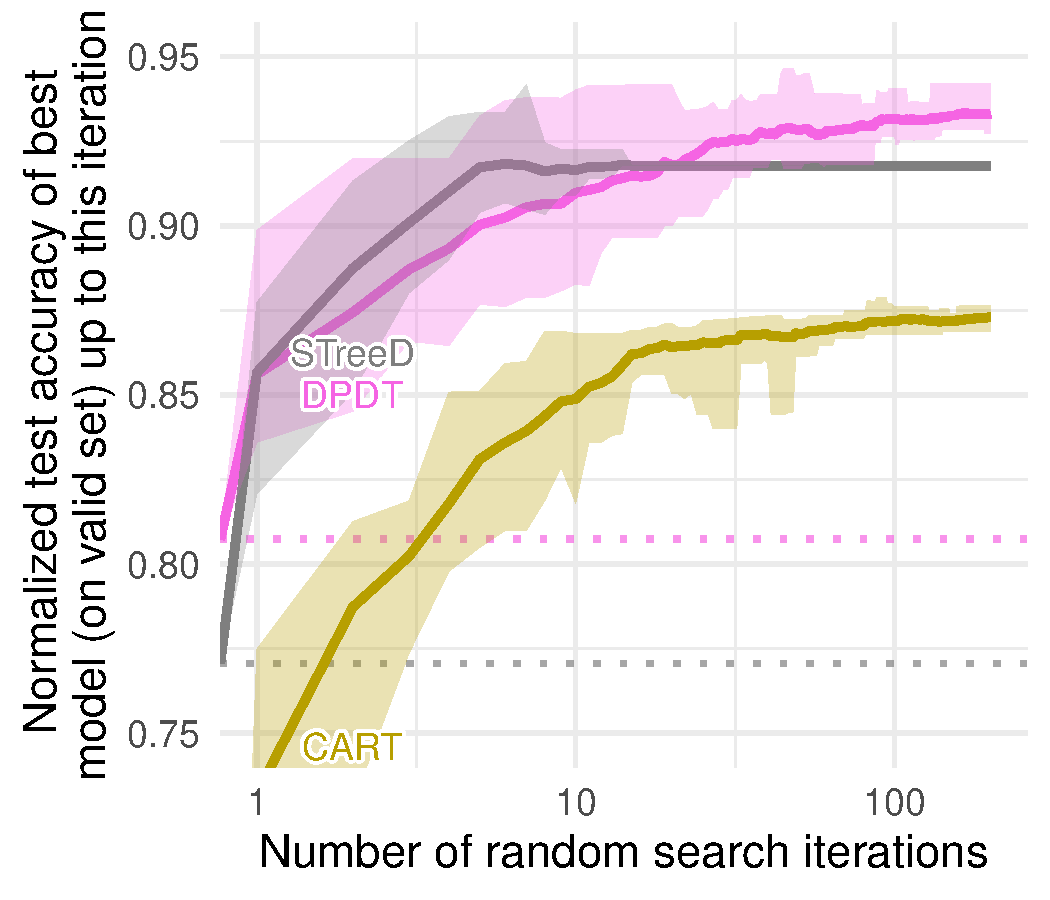
\includegraphics[width=\textwidth]{images/figures/tab_bench/random_search_classif_numerical_depth5.pdf}
        \subcaption{Single Tree Numerical}\label{fig:gen-num}
    \end{minipage}
    \begin{minipage}{0.24\textwidth}
        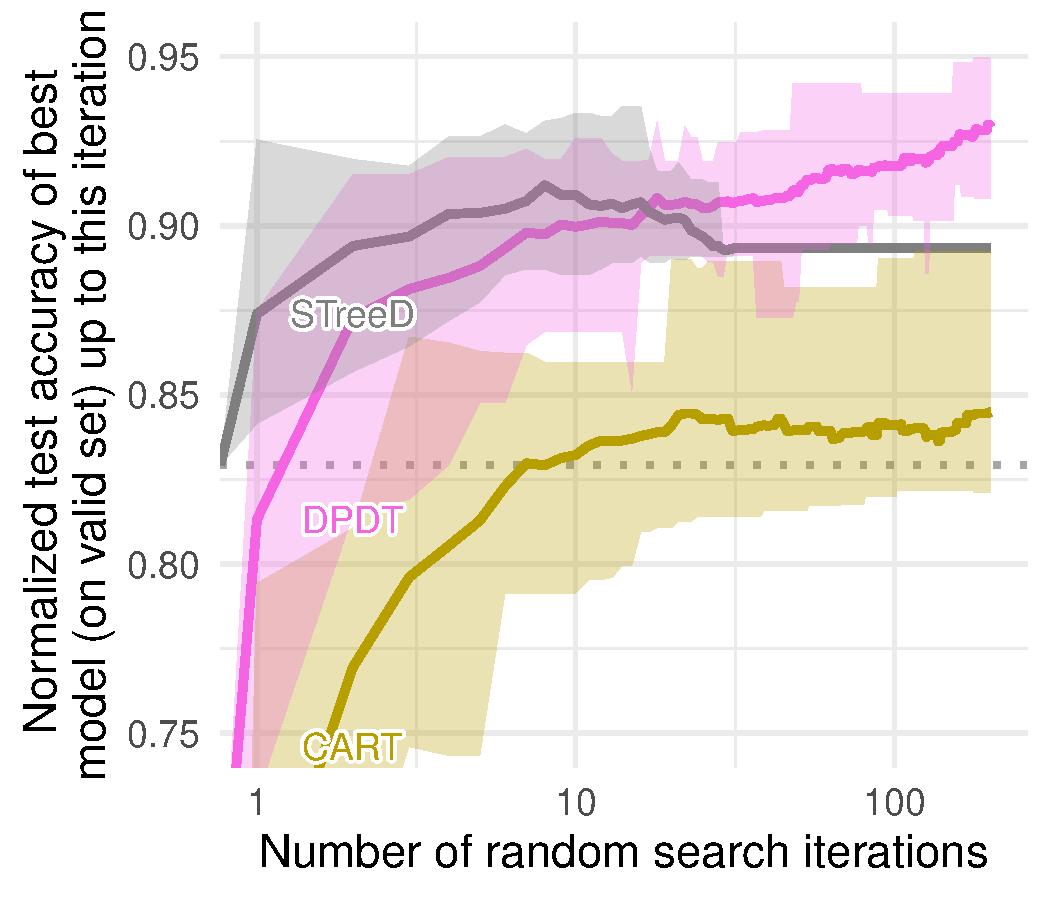
\includegraphics[width=\textwidth]{images/figures/tab_bench/random_search_classif_categorical_depth5.pdf}
        \subcaption{Single Tree Categorical}\label{fig:gen-cat}
    \end{minipage}
        \centering
    \begin{minipage}{0.24\textwidth}
        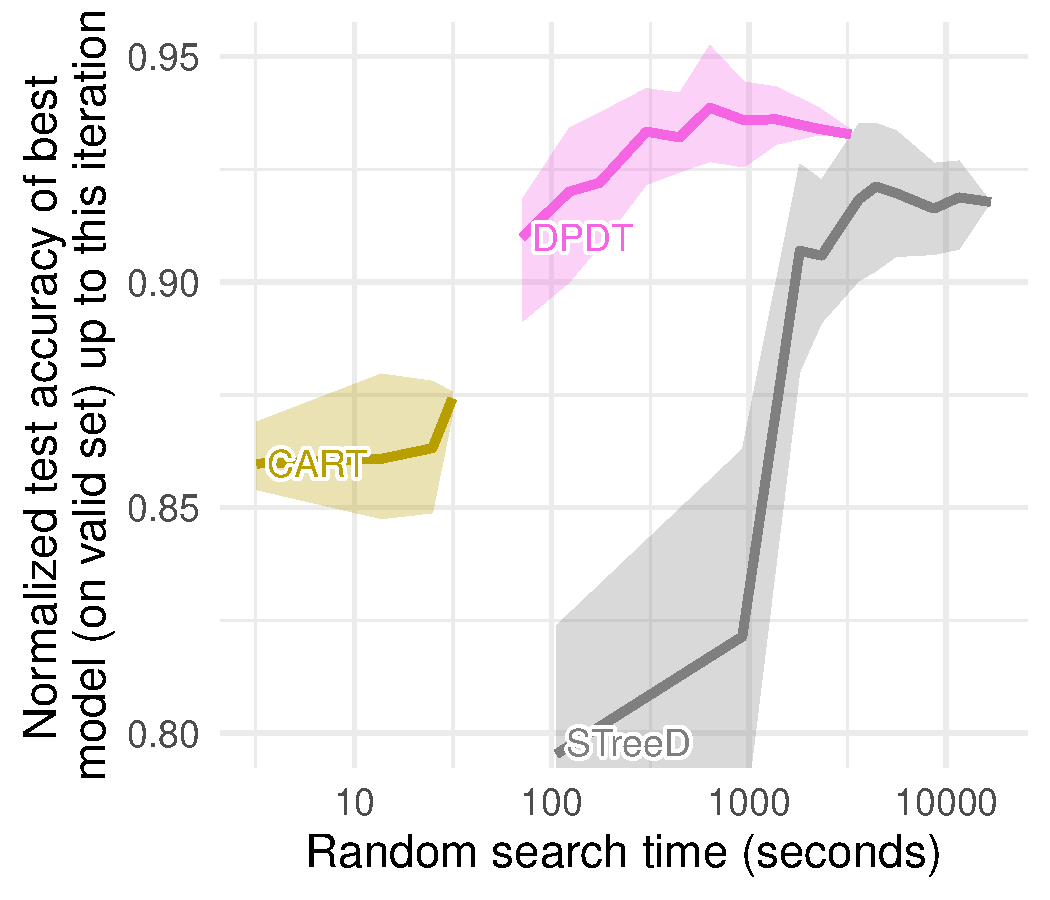
\includegraphics[width=\textwidth]{images/figures/tab_bench/benchmark_time_numerical_classif.pdf}
        \subcaption{Single Tree Numerical}\label{fig:gen-num-time}
    \end{minipage}
    \begin{minipage}{0.24\textwidth}
        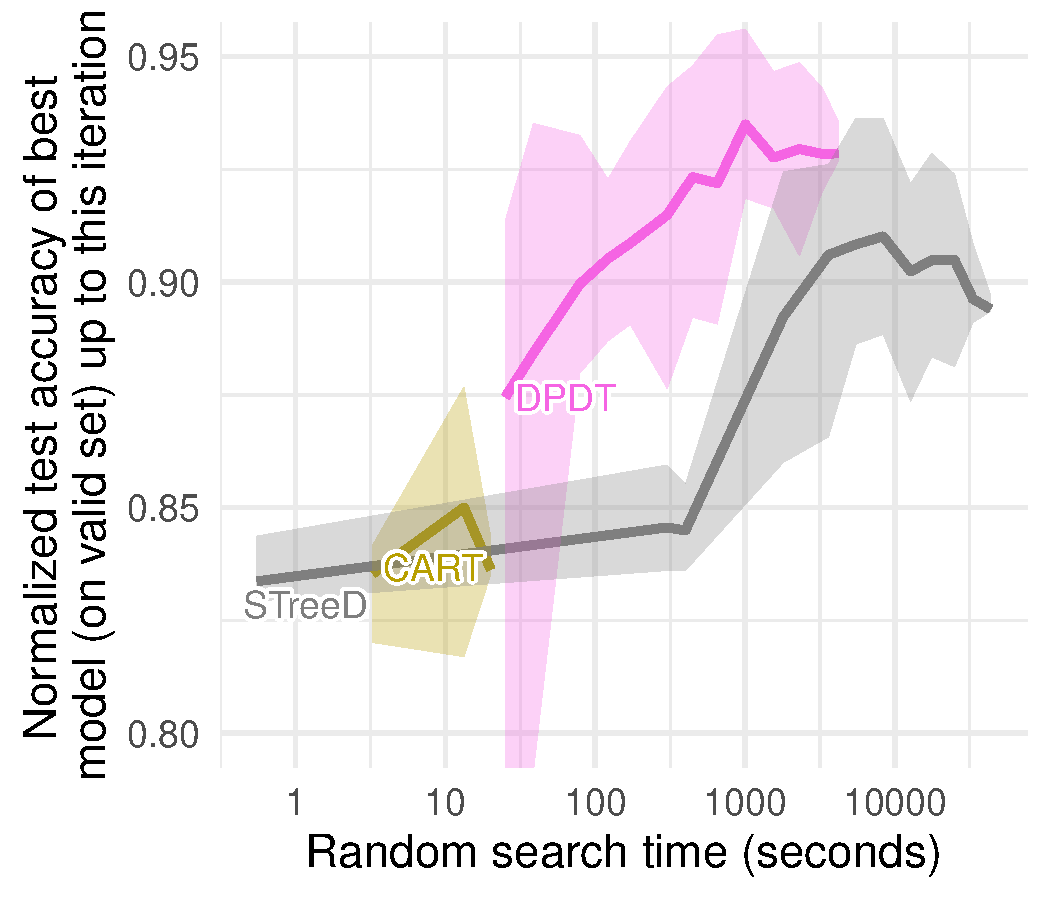
\includegraphics[width=\textwidth]{images/figures/tab_bench/benchmark_time_categorical_classif.pdf}
        \subcaption{Single Tree Categorical}\label{fig:gen-cat-time}
    \end{minipage}
          \begin{minipage}{0.24\textwidth}
          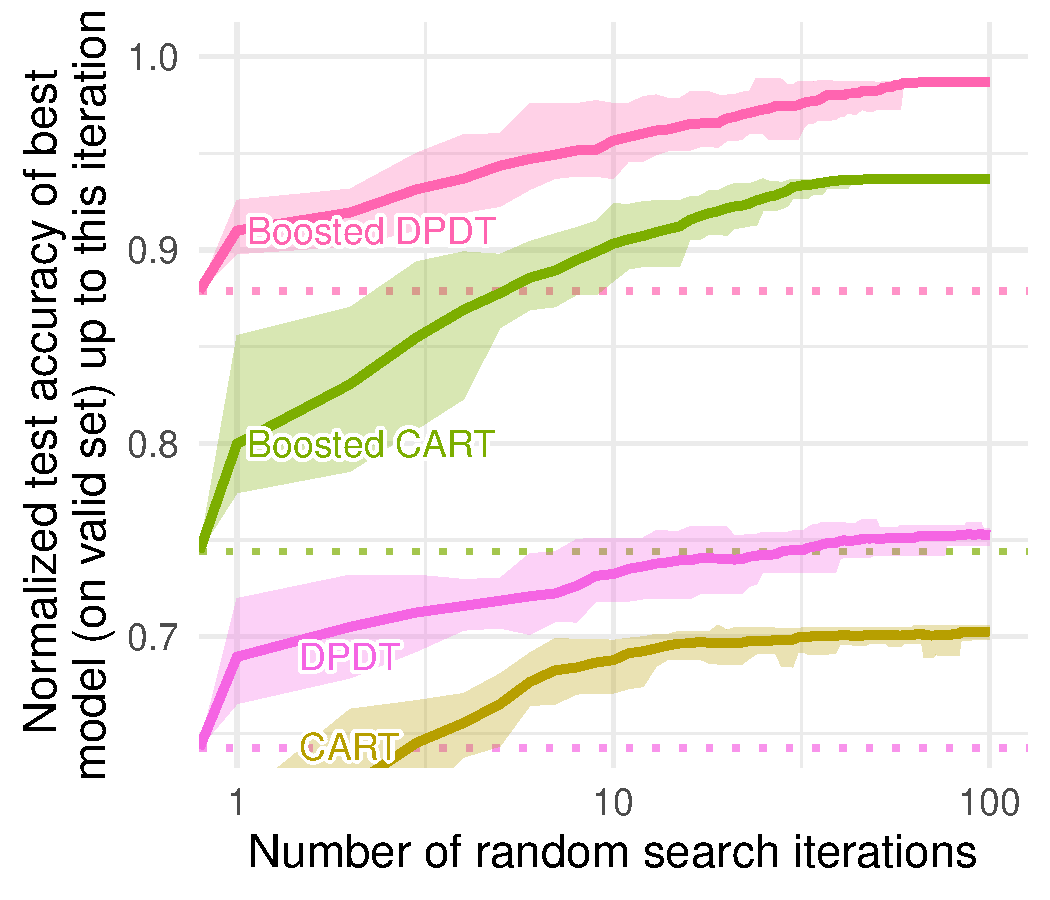
\includegraphics[width=\textwidth]{images/figures/tab_bench/random_search_classif_numerical_boosting_w_weak.pdf}
          \subcaption{Boosting vs Single Tree Num.}\label{fig:boost-num}
      \end{minipage}
      \begin{minipage}{0.24\textwidth}
          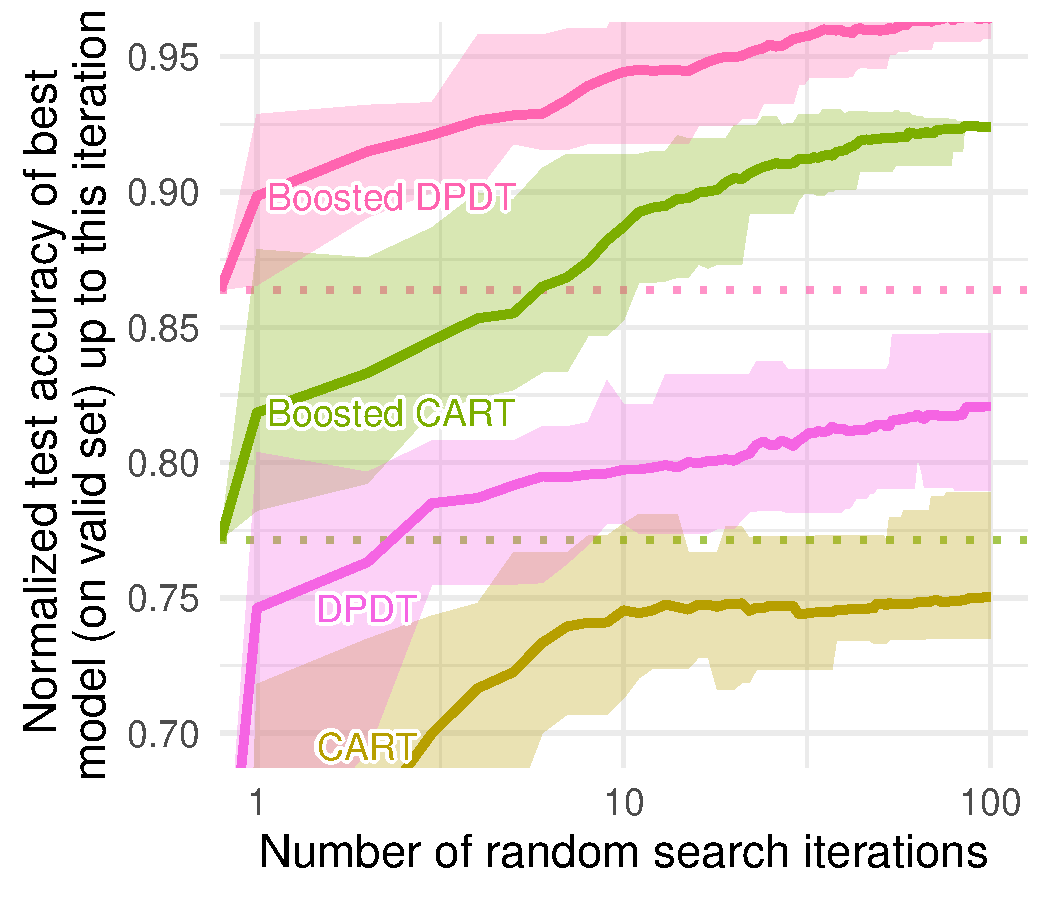
\includegraphics[width=\textwidth]{images/figures/tab_bench/random_search_classif_categorical_boosting_w_weak.pdf}
          \subcaption{Boosting vs Single Tree Cat.}\label{fig:boost-cat}
      \end{minipage}
    \centering
    \begin{minipage}{0.24\textwidth}
        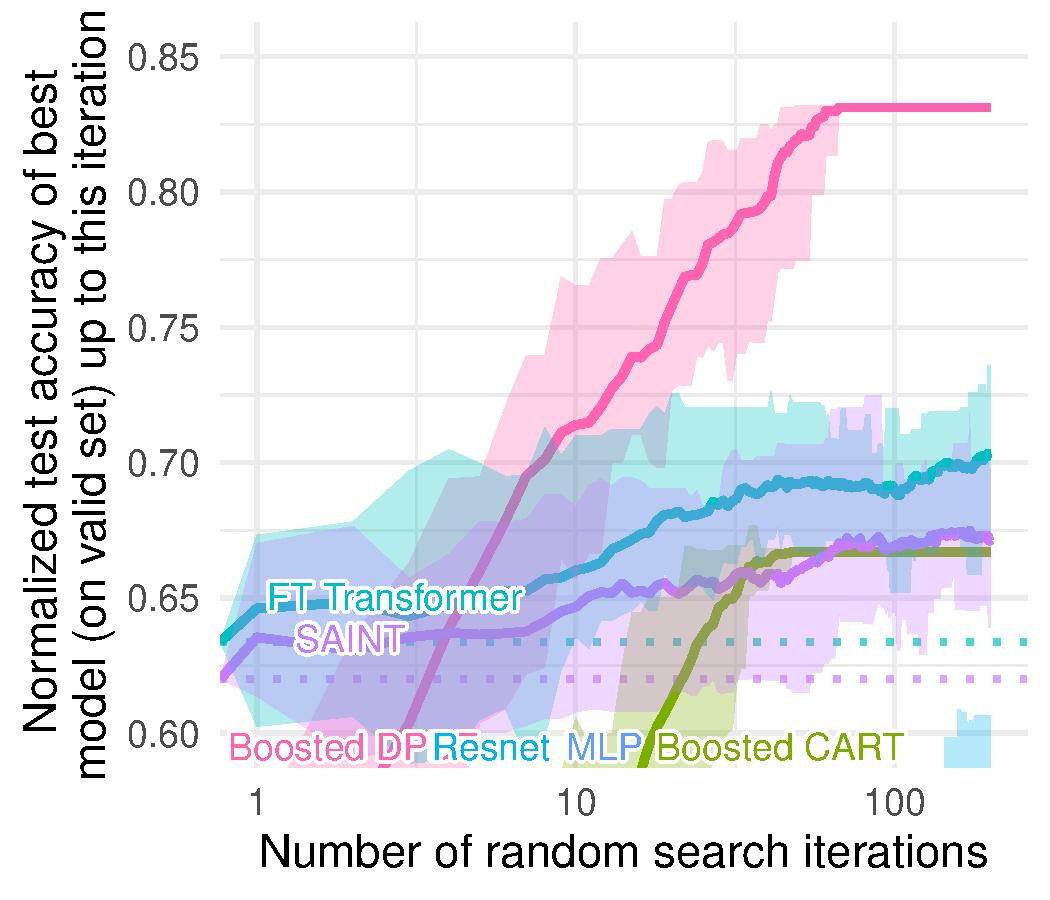
\includegraphics[width=\textwidth]{images/figures/tab_bench/random_search_classif_numerical_boosting_all_notgb.pdf}
        \subcaption{Boosting vs Neural Numerical}\label{fig:classif-num-all}
    \end{minipage}
    \begin{minipage}{0.24\textwidth}
        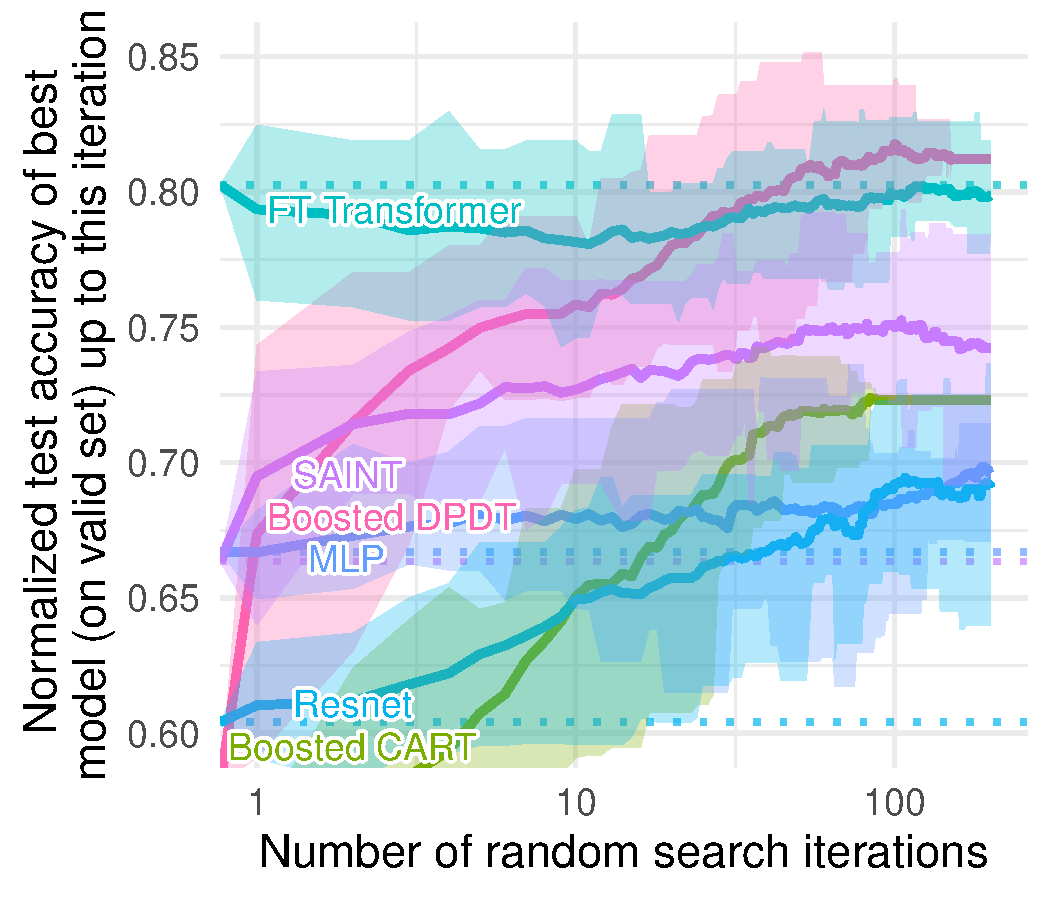
\includegraphics[width=\textwidth]{images/figures/tab_bench/random_search_classif_categorical_boosting_all_notgb.pdf}
        \subcaption{Boosting vs Neural Categorical}\label{fig:classif-cat-all}
    \end{minipage}
\caption{Benchmark on medium-sized datasets. Dotted lines correspond to the score of the default hyperparameters, which is also the first random search iteration. Each value corresponds to the test score of the best model (obtained on the validation set) after a specific number of random search iterations (a, b) or after a specific time spent doing random search (c, d), averaged on 15 shuffles of the random search order. The ribbon corresponds to the minimum and maximum scores on these 15 shuffles.}\label{fig:gen-classif}
\end{figure}

The goal of this section is to have a fair comparison of generalization capabilities of different tree induction algorithms. Fairness of comparison should take into account the number of hyperparameters, choice of programming language, intrinsic purposes of each algorithms (what are they designed to do?), the type of data they can read (categorical features or numerical features). We benchmark DPDT using~\cite{grinsztajn2022tree}. We choose this benchmark because it was used to establish XGBoost~\cite{xgb} as the SOTA tabular learning model. 

\subsection{Setup}

\paragraph{Metrics:} We re-use the code from \cite{grinsztajn2022tree}~\footnote{https://github.com/leogrin/tabular-benchmark}. It relies on random searches for hyper-parameter tuning \cite{pmlr-v28-bergstra13}. We run a random search of 100 iterations per dataset for each benchmarked tree algorithms. To study performance as a function of the number $n$ of random search iterations, we compute the best hyperparameter combination on the validation set on these $n$ iterations (for each model and dataset), and evaluate it on the test set. Following \cite{grinsztajn2022tree}, we do this 15 times while shuffling the random search order at each time. This gives us bootstrap-like estimates of the expected test score of the best tree found on the validation set after each number of random search iterations. In addition, we always start the random searches with the default hyperparameters of each tree induction aglorithm. We use the test set accuracy (classification) to measure model performance. The aggregation metric is discussed in details in \cite[section 3]{grinsztajn2022tree}.

\paragraph{Datasets:} we use the datasets curated by \cite{grinsztajn2022tree}. They are available on \texttt{OpenML} \cite{10.1145/2641190.2641198} and described in details in \cite[appendix A.1]{grinsztajn2022tree}. The attributes in these datasets are either %Those datasets are either 
numerical (a real number), or categorical (a symbolic values among a finite set of possible values). %,  strings as well as numbers). 
The considered datasets follow a strict selection \cite[section 3]{grinsztajn2022tree} to focus on core learning challenges. Some datasets are very large (millions of samples) like Higgs or Covertype \cite{higgs_280,covertype_31}. To ensure non-trivial learning tasks, datasets where simple models (e.g.\@ logistic regression) performed within 5\% of complex models (e.g.\@ ResNet~\cite{resnet}, HistGradientBoosting~\cite{scikit-learn}) are removed. We use the same data partitioning strategy as~\cite{grinsztajn2022tree}: 70\% of samples are allocated for training, with the remaining 30\% split between validation (30\%) and test (70\%) sets. Both validation and test sets are capped at 50,000 samples for computational efficiency. All algorithms and hyperparameter combinations were evaluated on identical folds. Finally, while we focus on classification datasets in the main text, we provide results for regression problems in table~\ref{tab:regression} in the appendix.

\paragraph{Baselines:}
we benchmark DPDT against CART and STreeD when inducing trees of depth at most 5.  We use hyperparameter search spaces from \cite{komer-proc-scipy-2014} for CART and DPDT. For DPDT we additionally consider eight different splits functions parameters configurations for the maximum nodes in the calls to CART. Surprisingly, after computing the importance of each hyperparameter of DPDT, we found that the maximum node numbers in the calls to CART are only the third most important hyperparametrer behind classical ones like the minimum size of leaf nodes or the minimum impurity decrease (Table~\ref{tab:importance_comparison}). We use the \texttt{CPython} implementation of STreeD\footnote{PySTreeD: \url{https://github.com/AlgTUDelft/pystreed}}. All hyperparameter grids are given in table \ref{tab:tree_hyperparams} in the appendix.

\paragraph{Hardware:} experiments were conducted on a heterogeneous computing infrastructure made of AMD EPYC 7742/7702 64-Core and Intel Xeon processors, with hardware allocation based on availability and algorithm requirements. DPDT and CART random searches ran for the equivalent of 2-days while \texttt{PySTreeD} ran for 10-days.

\begin{table}
\centering
\small
\caption{Hyperparameters importance comparison. A description of the hyperparameters can be found in the scikit-learn documentation: \url{https://scikit-learn.org/stable/modules/generated/sklearn.tree.DecisionTreeClassifier.html}.}
\begin{tabular}{lccc}
\toprule
\textbf{Hyperparameter} & \textbf{DPDT (\%)}  & \textbf{CART (\%)} & \textbf{STreeD (\%)} \\
\midrule
min\_samples\_leaf & 35.05 & 33.50 & 50.50 \\
min\_impurity\_decrease & 24.60 & 24.52 & - \\
cart\_nodes\_list & 15.96 & - & - \\
max\_features & 11.16 & 18.06 & - \\
max\_depth & 7.98 & 10.19 & 0.00 \\
max\_leaf\_nodes & - & 7.84 & - \\
min\_samples\_split & 2.67 & 2.75 & - \\
min\_weight\_fraction\_leaf & 2.58 & 3.14 & - \\
max\_num\_nodes & - & - & 27.51 \\
n\_thresholds & - & - & 21.98 \\
\bottomrule
\end{tabular}
\label{tab:importance_comparison}
\end{table}

\subsection{Observations}

\paragraph{Generalization} In figure \ref{fig:gen-classif}, we observe that DPDT learns better trees than CART and STreeD both in terms of generalization capabilities and in terms of computation cost. On figures \ref{fig:gen-num} and \ref{fig:gen-cat}, DPDT obtains best generalization scores for classification on numerical and categorical data after 100 iterations of random hyperparameters search over both CART and STreeD. Similarly, we also present generalization scores as a function of compute time (instead of random search iterations). On figures \ref{fig:gen-num-time} and \ref{fig:gen-cat-time}, despite being coded in the slowest language (\texttt{Python} vs. \texttt{CPython}), our implementation of DPDT finds the best overall model before all STreeD random searches even finish.
The results from figure \ref{fig:gen-classif} are appealing for machine learning practitioners and data scientists that have to do hyperparameters search to find good models for their data while having computation constrains.

Now that we have shown that DPDT is extremely efficient to learn shallow decision trees that generalize well to unseen data, it is fair to ask if DPDT can also learn deep trees on very large datasets.

\begin{table}
\centering
\caption{Depth-10 decision trees for the KDD 1999 cup dataset.}
\label{tab:model-comparison}
\small
\begin{tabular}{lccc}
\hline
\textbf{Model} & \textbf{Test Accuracy (\%)} & \textbf{Time (s)} & \textbf{Memory (MB)} \\
\hline
DPDT-(4,) & \textbf{91.30} & 339.85 & 5054 \\
DPDT-(4,4,) & \textbf{91.30} & 881.07 & 5054 \\
CART & 91.29 & 25.36 & 1835 \\
GOSDT-$\alpha=0.0005$& 65.47 & 5665.47 & 1167 \\
GOSDT-$\alpha=0.001$ & 65.45 & 5642.85 & 1167 \\
\hline
\end{tabular}
\end{table}

\paragraph{Deeper trees on bigger datasets} We also stress test DPDT by inducing deep trees of depth 10 for the KDD 1999 cup dataset\footnote{\url{http://kdd.ics.uci.edu/databases/kddcup99/kddcup99.html}}. The training set has 5 million rows and a mix of 80 continuous and categorical features representing network intrusions. We fit DPDT with 4 split candidates for the root node (DPDT-(4,)) and with 4 split candidates for the root and for each of the internal nodes at depth 1 (DPDT-(4,4,)). We compare DPDT to CART with a maximum depth of 10 and to GOSDT\footnote{Code available at: \url{https://github.com/ubc-systopia/gosdt-guesses}}~\cite{mctavish2022fast} with different regularization values $\alpha$. GOSDT first trains a tree ensemble to binarize a dataset and then solve for the optimal decision tree of depth 10 on the binarized problem. In Table~\ref{tab:model-comparison} we report the test accuracy of each tree on the KDD 1999 cup test set. We also report the memory peak during training and the training duration (all experiments are run on the same CPU). We observe that DPDT can improve over CART even for deep trees and large datasets while using reasonable time and memory. Furthermore, Table \ref{tab:model-comparison} highlights the limitation of optimal trees for practical problems when the dataset is not binary. We observed that GOSDT could not find a good binarization of the dataset even when increasing the budget of the tree ensemble up to the point where most of the computations are spent on fitting the ensemble (see more details about this phenomenon in \cite[section 5.3]{mctavish2022fast}). In table \ref{tab:more-res} in the appendix, we also show that DPDT performs better than optimal trees for natively binary datasets. In the next section we study the performance of boosted DPDT trees.

\section{Application of DPDT to Boosting}

In the race for machine learning algorithms for tabular data, boosting procedures are often considered the go-to methods for classification and regression problems. Boosting algorithms \cite{FREUND1997119,stcohFriedman,FriedmanBoosting} sequentially add weak learners to an ensemble called strong learner. The development of those boosting algorithms has focused on what data to train newly added weak learners \cite{stcohFriedman,FriedmanBoosting},  or on efficient implementation of those algorithms \cite{xgb,10.5555/3327757.3327770}. We show next that Boosted-DPDT (boosting DPDT trees with AdaBoost \cite{FREUND1997119}) improves over recent deep learning algorithms. 

\subsection{Boosted-DPDT}\label{sec:boosting}

We benchmark Boosted-DPDT with the same datasets, metrics, and hardware as in the previous section on single-tree training. Second, we verify the competitiveness of Boosted-DPDT with other models such as deep learning ones (SAINT~\cite{somepalli2021saintimprovedneuralnetworks} and other deep learning architectures from \cite{resnet}). 

On figures \ref{fig:boost-num} and \ref{fig:boost-cat} we can notice 2 properties of DPDT. First, as in any boosting procedure, Boosted-DPDT outperforms its weak counterpart DPDT. This serves as a sanity check for boosting DPDT trees. Second, it is clear that boosting DPDT trees yields better models than boosting CART trees on both numerical and categorical data. figures~\ref{fig:classif-num-all} and \ref{fig:classif-cat-all} show that boosting DPDT trees using the default AdaBoost procedure~\cite{FREUND1997119} is enough to learn models outperforming deep learning algorithms on datasets with numerical features and models in the top-tier on datasets with categorical features. This show great promise for models obtained when boosting DPDT trees with more advanced procedures.

\subsection{(X)GB-DPDT}
\begin{figure}
    \centering
    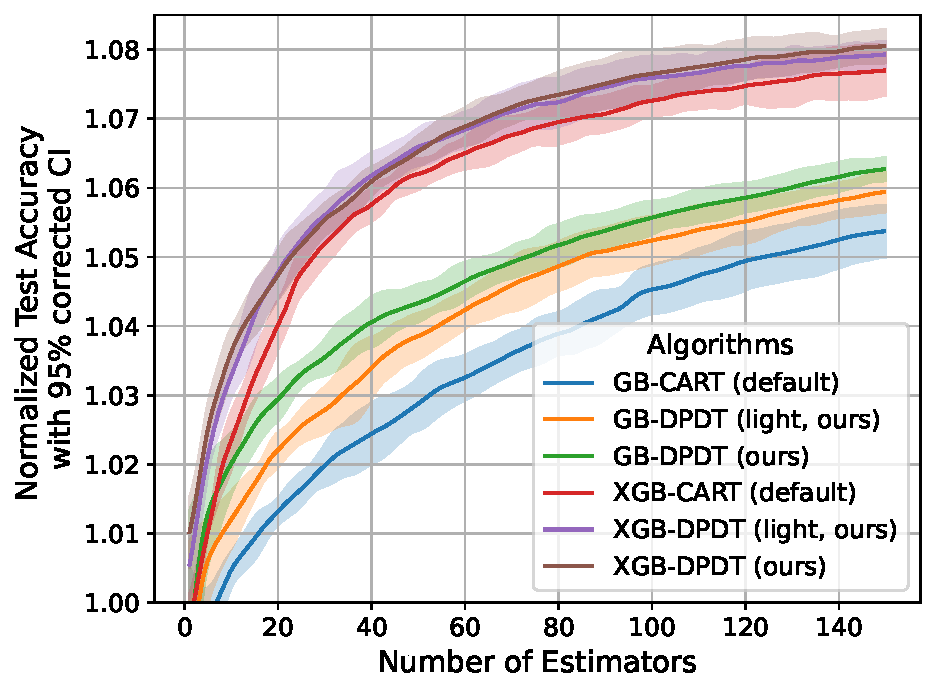
\includegraphics[trim={0 0 0 0},clip,width=0.6\linewidth]{images/figures/xgboosting_normalized_wo_opt.pdf}
    \caption{Aggregated mean test accuracies of Gradient Boosting models as a function of the number of single trees.}
    \label{fig:gb}
\end{figure}

We also boost DPDT trees with Gradient Boosting and eXtreme Gradient Boosting~\cite{FriedmanBoosting,stcohFriedman,xgb}(X(GB)-DPDT). For each dataset from~\cite{grinsztajn2022tree}, we trained (X)GB-DPDT models with 150 boosted single DPDT trees and a maximum depth of 3 for each. We evaluate two DPDT configurations for the single trees: light (DPDT-(4, 1, 1)) and the default (DPDT-(4,4,4)). We compare (X)GB-DPDT to (X)GB-CART: 150 boosted CART trees with maximum depth of 3 and default hyperparameters for each. All models use a learning rate of 0.1. For each each dataset, we normalize all boosted models scores by the accuracy of a single depth-3 CART decision tree and aggregate the results: the final curves represent the mean performance across all datasets, with confidence intervals computed using 5 different random seeds.

figure~\ref{fig:gb} shows that similarly to simple boosting procedures like AdaBoost, more advanced ones like (eXtreme) Gradient Boosting yields better models when the weak learners are DPDT trees rather than greedy trees. This is a motivation to develop efficient implementation of (eXtreme) Gradient Boosting with DPDT as the weak learning algorithm to perform extensive benchmarking following \cite{grinsztajn2022tree} and potentially claim the state-of-the-art.



\section{Conclusion}\label{sec:ccl-dpdt}

In this part of the manuscript, we introduced Dynamic Programming Decision Trees (DPDT), a novel framework that bridges the gap between greedy and optimal decision tree algorithms. By formulating tree induction as an MDP and employing adaptive split generation based on CART, DPDT achieves near-optimal training loss with significantly reduced computational complexity compared to existing optimal tree solvers. Furthermore, we prove that DPDT can learn strictly more accurate trees than CART. 
Most importantly, extensive benchmarking on varied large and difficult enough datasets showed that DPDT trees and boosted DPDT trees generalize better than other baselines. To conclude, we showed that DPDT is a promising machine learning algorithm. 

The key future work would be to make DPDT industry-ready by implementing it in \texttt{C} and or making it compatible with the most advanced implementation of e.g.\@ XGBoost.
While DPDT is designed for supervised learning (\ref{sec:dl}), an other interesting future work direction could be to use DPDT in the tree induction routine of imitation learning algorithms like VIPER (algorithm~\ref{alg:viper},~\cite{viper}).
This could lean to better decision tree policy learning for the RL objective (\ref{def:mdp-obj}).

In the next and final part of this manuscript, we circle back to our original sequential decision making problems.
We will move away from \textit{learning} and focus on evaluating the interpretability-performance trade-offs of different policy class from figure~\ref{fig:performance-interpretability-trade-off}.
